\documentclass[10pt]{report}
\usepackage[utf8]{inputenc}
\usepackage[italian]{babel}
\usepackage{multicol}
\usepackage[bookmarks]{hyperref}
\usepackage[a4paper, total={18cm, 25cm}]{geometry}
\usepackage{graphicx}
\usepackage{xcolor}
\usepackage{textcomp}
\graphicspath{ {./img/} }
\usepackage{listings}
\usepackage{makecell}
\usepackage{qtree}
\usepackage{pgfplots}
\usepackage{tikz}
\usepgflibrary{shapes}
\usepgfplotslibrary{fillbetween}
\definecolor{backcolour}{RGB}{255,255,255}
\definecolor{codegreen}{RGB}{27,168,11}
\definecolor{codeblue}{RGB}{35,35,205}
\definecolor{codegray}{RGB}{128,128,128}
\definecolor{codepurple}{RGB}{205,35,56}
\lstdefinestyle{myPython}{
	backgroundcolor=\color{backcolour},   
	commentstyle=\color{codegreen},
	keywordstyle=\color{codeblue},
	numberstyle=\tiny\color{codegray},
	stringstyle=\color{codepurple},
	basicstyle=\small\ttfamily,
	breakatwhitespace=false,         
	breaklines=true,                 
	captionpos=b,                    
	keepspaces=true,                 
	numbers=left,                    
	numbersep=2pt,                  
	showspaces=false,                
	showstringspaces=false,
	showtabs=false,                  
	tabsize=2,
	language=python
}
\newcommand*\triangled[1]{\tikz[baseline=(char.base)]{
            \node[regular polygon, regular polygon sides=3,draw,inner sep=1pt] (char) {#1};}}
            
\usepackage{fancyhdr}
\pagestyle{fancy}
\renewcommand{\headrulewidth}{0pt}
\fancyhead{}
\fancyfoot[L]{Telegram: \texttt{@fexed}}
\fancyfoot[R]{Github: \texttt{fexed}}
\begin{document}
\title{Intelligent Systems for Pattern Recognition}
\author{Federico Matteoni}
\date{A.A. 2021/22}
\renewcommand*\contentsname{Index}

\maketitle
\tableofcontents
\pagebreak
\section{Introduction}
Prof.s: Davide Bacciu and Antonio Carta
\paragraph{Objectives} Train ML specialists capable of: designing novel learning models, developing pattern recognition applications using ML, developing intelligent agents using \textbf{Reinforcement Learning}.\\
We're referring to images and signals, but not limited to that: practical applications.\\
Focusing on challenging and complex data: \textbf{machine vision} (noisy, hard to interpret, semantically rich\ldots) and \textbf{structured data} (relational information: sequences, trees, graphs\ldots)\\
Natural Language Processing will be used as an example, but will not be the focus of this course.
\paragraph{Methodology-Oriented Outcomes} Gain in-depth knowledge of advanced machine learning models, understanding the underlying theory. This gives the ability to read and understand and discuss research works in the field.
\paragraph{Application-Oriented Outcomes} Learn to address modern pattern recognition applications, gain knowledge of ML, PR and RL libraries and be able to develop an application using ML and RL models.
\paragraph{Prerequisites} Knowledge of ML fundamentals, mathematical tools for ML and Python.
\section{Pattern Recognition}
Automated recognition of meaningful patterns in noisy data.
\paragraph{Origins} 
\paragraph{Viola-Jones Algorithm} Framework for face recognition. Sum pixel in white area and subtract those in the black portion. The VJ algorithm positions the masks on the image and combines the responses (training set of $\simeq$5k images with hand-aligned filters)
\paragraph{An historical view} \begin{enumerate}
	\item Identification of distinguishing features of the object/entity (\textbf{feature detection})
	\item Extraction of features for the defining attributes (\textbf{feature extraction})
	\item Comparison with known patterns (\textbf{matching})
\end{enumerate}
Basically, lots of time spent hand-engineering the best data features.
\paragraph{A modern view}
Data is thrown into a neural network. A single stage process with a data crushing-and-munching neural network spitting out prediction, which encapsulates the three historical steps. But the time is now spent in fine-tuning the neural network.
\paragraph{The deep learning Lego} Creating applications by putting together various combinations of CNN and LSTM modules.
\subsection{Signals}
Signals are time series: a sequence of measurements in time. Examples of sources are: medicine, finance, geology, IoT, biometrics\ldots
\paragraph{Formalization} A time series x is a sequence of measurements in time $t$
$$\hbox{x} = x_0,\ldots,x_N$$
where $x_t$ or $x(t)$ is the measurement at time $t$.
\begin{list}{}{}
	\item Observation can be at \textbf{irregular} time intervals.
	\item We assume \textbf{weakly stationary} (or second-order stationary) data\begin{list}{}{}
		\item $\forall\:t\:\:E[x_t] = \mu$
		\item $\forall\:t$ Cov$(x_{t+\tau},x_t) = \gamma_\tau$ with $\gamma$ depending only on the lag $\tau$
	\end{list}
\end{list}
\paragraph{Goals}\begin{list}{}{}
	\item \textbf{Description}
	\item \textbf{Analysis}: identify and describe dependencies in data
	\item \textbf{Prediction}: forecast next values given information up to $t$
	\item \textbf{Control}: adjust parameters of the generative process to make the time series fit a target
\end{list}
\paragraph{Key Methods}\begin{list}{}{}
	\item \textbf{Time domain analysis}: assesses how a signal changes over time (correlation, convolution, auto-regressive models)
	\item \textbf{Spectral domain analysis}: assesses the distribution of the signal over a range of frequencies (Fourier analysis, wavelets)
\end{list}
\subsubsection{Time Domain Analysis}
\paragraph{Mean} $$\hat\mu=\frac{1}{N}\sum_{t=1}^N x_t$$
Can be used to subtract mean from values and "standardize" the two series.
\paragraph{Autocovariance} For lag $-N\leq \tau \leq N$
$$\hat\gamma_x(\tau) = \frac{1}{N}\sum_{t=1}^{N-|\tau|} (x_{t+|\tau|}-\hat\mu)(x_t - \hat\mu)$$
\paragraph{Autocorrelation} The correlation of a signal with itself. $$\hat\rho_x(\tau)=\frac{\hat\gamma_x(\tau)}{\hat\gamma_x(0)}$$
We can compute this with every possible $\tau$, finding the max/min which gives the $\tau$ where the autocorrelation is max/min, which means the lag where the signal starts repeating itself. The lags near zero typically dominates, so we want the maximum lag reasonably far from 0.
\subparagraph{Autocorrelation plot} %TODO
\paragraph{Cross-Correlation} A measure of similarity of x$_1$ and x$_2$ as a function of a time lag $\tau$ $$\phi_{\hbox{x}_1\:\hbox{x}_2}(\tau)=\sum_{t = \max\{0,\tau\}}^{\min\{(T_1 - 1 + \tau), (T_2 - 1)\}} \hbox{x}_1(t-\tau)\cdot \hbox{x}_2(t)$$
\subparagraph{Normalized cross-correlation} Returns an amplitude independent value %TODO
$$\overline{\phi}_{\hbox{x}_1\:\hbox{x}:2}(\tau) = \frac{\phi_{\hbox{x}_1\:\hbox{x}:2}}{\hbox{\texttt{todo}}} \in [-1,+1]$$
With $\overline{\phi}_{\hbox{x}_1\:\hbox{x}:2}(\tau) = +1$ mean that the two time series have the exact same shape if aligned at time $\tau$. Nearing $-1$ we get the maximum anticorrelation, same shape but opposite sign. Near 0 we get that the two signals are completely \textbf{linearly} uncorrelated.\\
Note that we measure \textbf{linear correlation}.\\\\
Cross correlation looks like the convolution $$(f * g)[n]=\sum_{t=-M}^M f(n-t)g(t)$$ but we have a flipped sign ($n-t$ instead of $t-\tau$).\\
Cross-correlation is not symmetric, whereas convolution is ($f * g = g * f$).
\paragraph{Autoregressive Process} A timeseries autoregressive process (AR) of order $K$ is the linear system $$x_t = \sum_{k=1}^K \alpha_k x_{t-k} + \epsilon_t$$\begin{list}{}{}
	\item Autoregressive means $x_t$ regresses on itself
	\item $\alpha_k \Rightarrow$ linear coefficients$\:|\:|\alpha|<1$
	\item $\epsilon_t\Rightarrow$ sequence of independent and identically distributed values with mean 0 and fixed variance.
	\item We look backward $K$ steps, so limited memory.
\end{list}
\paragraph{ARMA} Autoregressive with Moving Average process $$x_t = \sum_{k=1}^K \alpha_k x_{t-k} + \sum_{q=1}^Q \beta_q\epsilon_{t-1}+\epsilon_t$$
\begin{list}{}{}
	\item With $\epsilon_t$ Random white noise (again)
	\item The current time series values is the result of a regression on its past values plus a term that depends on a combination of stochastically uncorrelated information
\end{list}
\paragraph{Estimating Autoregressive Models} Need to estimate: the values of the linear coefficients $\alpha_t$ and $\beta_t$ and the order of the autoregressor $K$ and $Q$\\
Estimation of the $\alpha$, $\beta$ is performed with the Levinson-Durbin Recursion (\texttt{levinson(x, K)} in matlab, and included in several Python modules).\\
The order is often estimated with a Bayesian model selection criterion, choosing the largest $K$ and $Q$ possible. E.g.: BIC, AIC\ldots\\
The set of autoregressive parameters $\alpha_{i,1},\ldots,\alpha_{i,K}$ fitted to a specific time series x$_i$ is used to confront it with other time series. Same thing for $\beta$ so we can use $\alpha$ for both sets.
\paragraph{Comparing time series by AR}\begin{list}{}{}
	\item timeseries clustering %TODO
	\item novelty/anomaly detection %TODO
\end{list}
\subsubsection{Spectral Domain Analysis}
Analyze the time series in the frequency domain. Key idea: decomposing the time series into a linear combination of sines and cosines with random and uncorrelated coefficients. So a \textbf{regression on sinusoids} with Fourier analysis.
\paragraph{Fourier Transform} Discrete Fourier Transform (DFT): transform a time series from the time domain to the frequency domain. Can be easily inverted back to the time domain.\\
Useful to handle periodicity in the time series: seasonal trends, cyclic processes\ldots
\paragraph{Representing functions} We know that, given an orthonormal system for $E$ we can use linear combinations of the basis $\{e_1,\ldots\}$ to represent any function $f\in E$ $$\sum_{k=1}^\infty \langle f,e_k\rangle e_k$$
Given the orthonormal system $$\{\frac{1}{\sqrt{2}}, \sin(x),\cos(x),\sin(2x),\cos(2x),\ldots\}$$
The linear combination above becomes the Fourier series \texttt{todo} %TODO
\paragraph{Representing function in Complex space} Using $\cos(kx)-i\:\sin(kx) = e^{-ikx}$ with $i=\sqrt{-1}$ we can rewrite the Fourier series as $$\sum_{k=-\infty}^\infty c_k e^{ikx}$$
on the orthonormal system $$\{1,e^{ix},e^{-ix},e^{2ix},e^{-2ix},\ldots\}$$
\paragraph{Representing Discrete Time Series} Consider x of length $N$ and $x_n\in R$. Using the exponential formulation, the orthonormal system is finite, from $e_0$ to $e_{N-1}$ each $\in C^N$\\
The $n$-th component of the $k$-th vector is $$[e_k]n=e^{\frac{-2\pi ink}{2}}$$
\paragraph{Discrete Fourier Transform} Given a time series x = $x_0,\ldots,x_{N-1}$ its DFT is the sequence $$\hbox{Spectral domain}\:\:\:X_k = \sum_{n=1}^{N-1}x_ne^{\frac{-2\pi ink}{N}}\:\:\:\hbox{Time domain}$$
And can be inverted $$x_k = \frac{1}{N}\sum_{k=1}^{N-1}X_ke^{\frac{2\pi ink}{N}}$$
\paragraph{Basic Spectral Quantities in SFT}
\begin{list}{}{}
	\item Amplitude $A_k = |X_k| = \sqrt{Re^2(X_k)+Im^2(X_k)}$
	\item Power $P_k = \frac{|X_k|^2}{N}$, more used in reality and under some conditions this is a reasonable estimate of %TODO
\end{list}
\paragraph{DFT in Action} We use the DFT elements $X_1,\ldots,X_K$ as representation of the signal to train the predictor/classifier.\\
This representation can reveal patterns that are not clear in the time domain.
\subsection{Image Processing}
Bidimentional series. Basically same approach to signals.
\subsubsection{Descriptors}
An image is a matrix of pixel intensities or color values (RGB). There are other representations, not interesting for this course. CIE-LUV often used in image processing due to perceptual linearity (image difference is more coherent)
\paragraph{Machine Vision Applications} For example region of interest, or object classification.\\
Even pixel-level tasks, for example image segmentation (regions of the image) or semantic segmentation (classifying regions of the image).\\
Up one level of abstraction: automated image captioning, requiring identifying objects, generating sentences and ranking those sentences.
\paragraph{Key Questions}
\begin{list}{}{}
	\item How to represent visual information? It has to be:\begin{list}{}{}
		\item Informative, carrying all the information
		\item Invariant to photometric (different illuminations) and geometric transformation (position in the picture, rotation\ldots)
		\item Efficient for indexing and querying
	\end{list}
	\item How to identify informative parts?\begin{list}{}{}
		\item Whole image is generally not a good idea
		\item Must lead to good representations
	\end{list}
\end{list}
\paragraph{Image Histograms} One of the first answer. Describes the distribution of some visual information on the whole image: colors, edges, corners\ldots depending on the goals.\begin{list}{}{}
	\item \textbf{Color Histograms}, one of the earliest image descriptors.\\
	Count the number of pixels of a given color (normalize!). We need to discretize and group the RGB colors.\\
	Any information concerning shapes and position is lost. Two image with a random permutation of the same pixels produce the same color histograms.\\
	Images can be compared, indexed and classified based on their color histogram representation.\\
	Can be computed with OpenCV in Python.
\end{list}
\paragraph{Describing Local Image Properties} We need something less global, on a local level. Capturing information on image regions, extract \textbf{multiple local descriptors}: different location, different scale\ldots\\
Several approaches, typically performing convolution between a filter and the image region. Using filters sensitive to specific features we can extract many kind of information.
\paragraph{Localized Descriptors}
\begin{list}{}{}
	\item \textbf{Intensity Vector} The simplest form of localized descriptor: a vector $n\cdot m$ of the pixels of a single patch of the image with dimensions $n,m$. The vector can be normalized to make it invariant to intensity variations.\\
	But rotating gives a different vector. A more robust representation is an histogram of this vector.
	\item \textbf{Distribution-Based Descriptors} Represent local patches by histograms describing properties of the pixels in the patch. The simplest is an histogram of intensity values, but it's not invariant enough even if normalized.\\
	We want a descriptor invariant to illumination (normalization), scale (captured at multiple scale) and geometric transformations (rotation invariant). We want locality, histogram based and invariant to geometric transformation.
\end{list}
\paragraph{SIFT} \textbf{Scale Invariant Feature Transform}\begin{enumerate}
	\item Center the image patch on a pixel $x,y$ of the image $I$
	\item Represent image at scale $\sigma$ (controls how close to look at the image)
	\item[] Convolve the image with a Gaussian filter with standard variation $\sigma$, basically computing average of pixels with the coefficient taken from a Gaussian distribution. With a smooth Gaussian, we artificially smooth the object, and vice versa. We can compute different versions of the image.
$$L_\sigma(x,y) = G(x,y,\sigma) * I(x,y)$$
$$G(x,y,\sigma) = \exp\left(-\frac{x^2+y^2}{2\sigma^2}\right)$$
	\item Compute the \textbf{gradient of intensity} in the patch, extracting magnitude $m$ and orientation $\Theta$ using finite differences.
\end{enumerate}
\subparagraph{Gaussian Filter of an Image}
\begin{center}
	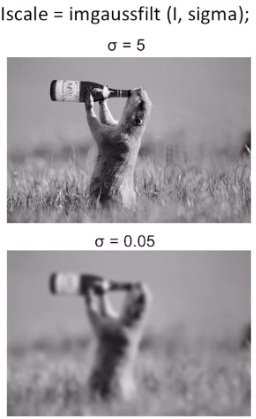
\includegraphics[scale=0.5]{1.png} 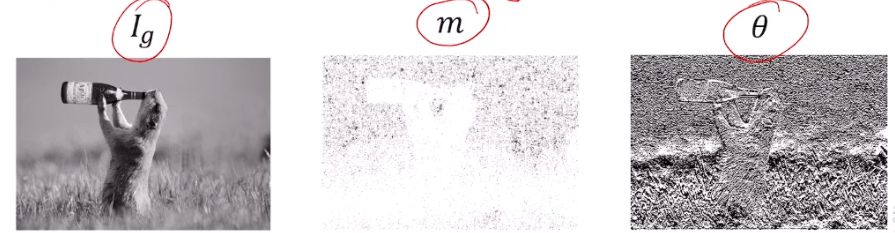
\includegraphics[scale=0.6]{2.png}
\end{center}
\pagebreak
\begin{list}{}{}
	\item[4.] Create \textbf{gradient histogram}\begin{list}{}{}
		\item 4$\times$4 gradient window
		\item Histogram of 4$\times$4 per window on 8 orientation bins
		\item Gaussian weighting on center keypoint (width = $1.5\sigma$)
		\item 4$\times$4$\times$8 = 128 descriptor size
	\end{list}
\end{list}
\begin{center}
	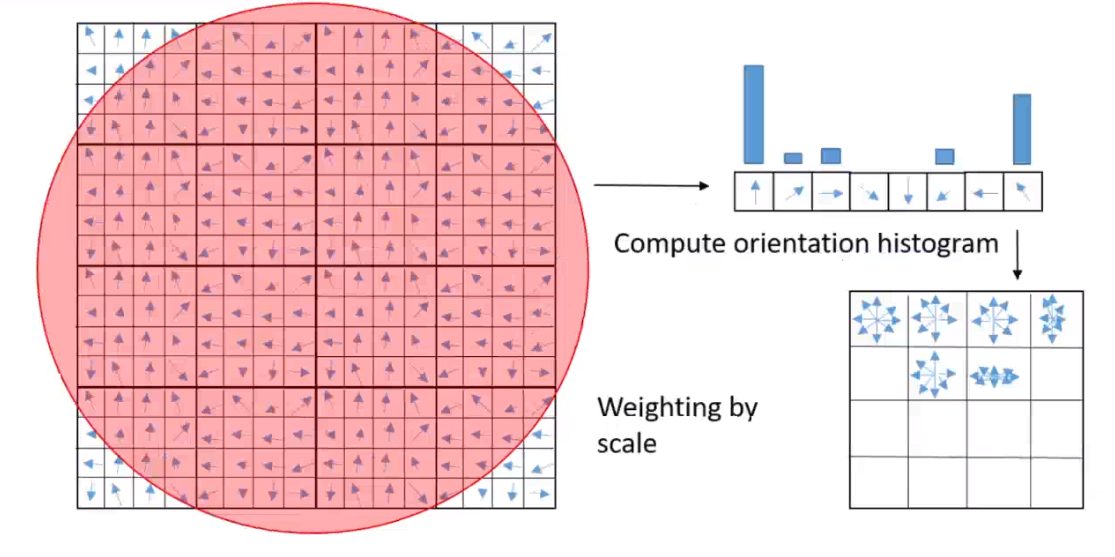
\includegraphics[scale=0.5]{3.png}
\end{center}
\subsubsection{Detectors}
\paragraph{Visual Feature Detector} Properties
\begin{list}{}{}
	\item \textbf{Repeatability} Detect the same feature in different image portions and different images, under different conditions (color, luminance\ldots). So with respect to translation, photometric changes, rotation, scaling and affine transformations (non-isotropic changes, for example the relative position of the camera)\ldots
\end{list}
\paragraph{Edge Detection} We need to find interesting points, talking about fundamental elements, basic components. One possible example are the edges of the image.\\
Reasoning in changes of intensity: edges are those points where the intensity changes.\begin{center}
	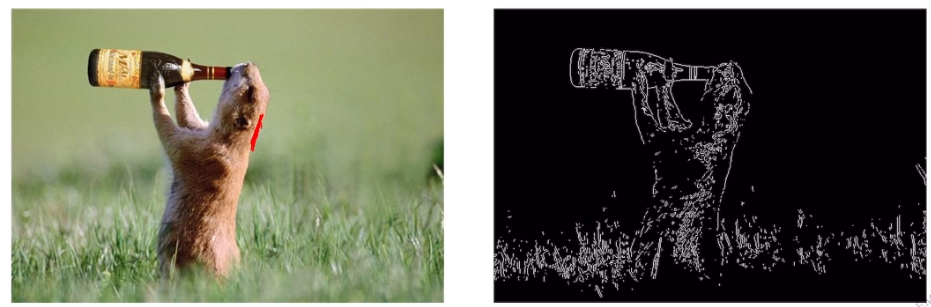
\includegraphics[scale=0.5]{4.png}
\end{center}
Typically using an edge detector filter on each pixel and turning pixels white or black by thresholding
\subparagraph{Edges and Gradients} The image gradient (graylevel) is $$\nabla I = \left[\frac{\partial I}{\partial x},\frac{\partial I}{\partial y}\right]$$ which is basically two images, gradient in both $x$ and $y$ directions. Edge are pixel regions where intensity gradient changes abruptly. The return of finite difference methods:
\begin{list}{}{}
	\item $G_x = \frac{\partial I}{\partial x} \simeq I(x+1,y)-I(x-1,y)$
	\item $G_y = \frac{\partial I}{\partial y} \simeq I(x,y+1)-I(x,y-1)$
\end{list}
\pagebreak
Edge detectors build on this idea combining with some smoothing: average on multiple pixels.
\subparagraph{Prewitt operators}
$$G_x = \left[\begin{array}{c c c }
+1&0&-1\\
+1&0&-1\\
+1&0&-1
\end{array}\right]\:\:\:\:\:G_y = \left[\begin{array}{c c c }
+1&+1&+1\\
0&0&0\\
-1&-1&-1
\end{array}\right]$$
\begin{center}
	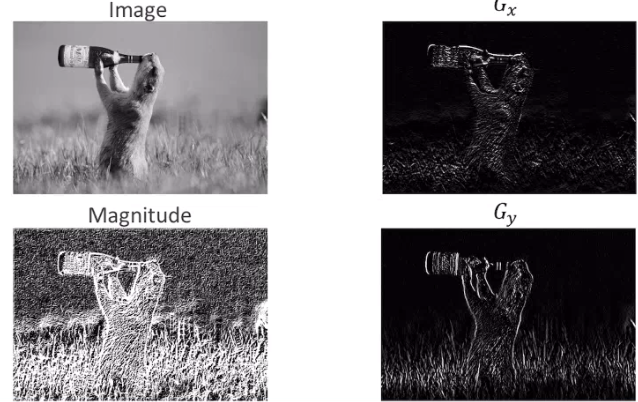
\includegraphics[scale=0.5]{5.png}
\end{center}
\subparagraph{Sobel Operator}
$$G_x = \left[\begin{array}{c c c }
+1&0&-1\\
+2&0&-2\\
+1&0&-1
\end{array}\right]\:\:\:\:\:G_y = \left[\begin{array}{c c c }
+1&+2&+1\\
0&0&0\\
-1&-2&-1
\end{array}\right]$$
Often with a constant $c\simeq \frac{1}{8}$ for scaling.
\begin{center}
	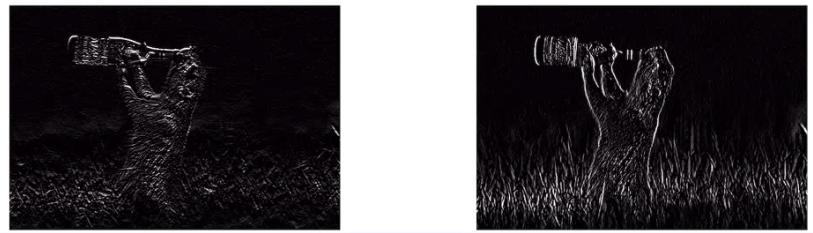
\includegraphics[scale=0.4]{6.png}
\end{center}
\paragraph{Blob Detection} Pixel regions with little gradient variability.\\
$g_\sigma(x,y)$ has maximum response when centered on a circle of radius $\sqrt{2}\sigma$, with $\sigma$ being the scale of the gaussian.\\
Laplace of Gaussian (LoG):
$$\nabla^2g_\sigma(x,y)=\frac{\partial^2g_\sigma}{\partial x^2} + \frac{\partial^2g_\sigma}{\partial y^2}$$
Typically using a scale normalized response
$$\nabla^2_{norm}g_\sigma(x,y)=\sigma^2\left(\frac{\partial^2g_\sigma}{\partial x^2} + \frac{\partial^2g_\sigma}{\partial y^2}\right)$$
\begin{enumerate}
	\item Convolve image with a LoG filter at different scales $\sigma = k\sigma_0$ by varying $k$ with a starting $\sigma_0$
	\item Find maxima of squared LoG responses:
	\begin{list}{}{}
		\item Find maxima on space-scale: focus on a scale and find maxima
		\item Find maxima between scales: do the same for all the scales and pick the maxima
		\item Threshold
	\end{list}
\end{enumerate}
The LoG can be approximated by the Difference of Gaussians (DoG) for efficiency, so to reuse part of the computations.
$$g_{k\sigma_0}(x,y) - g_{\sigma_0}(x,y) \simeq (k-1)\sigma_0^2\nabla^2g_{(k-1)\sigma_0}$$
SIFT uses LoG.
\paragraph{Affine Detectors} Laplacia-based detectors are invariant to scale thanks to the maximization in scale-space. Still not invariant to affine-transformation.
\begin{center}
	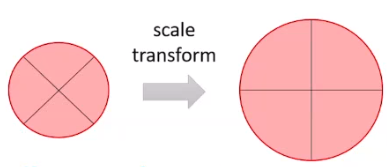
\includegraphics[scale=0.5]{7.png}\\
	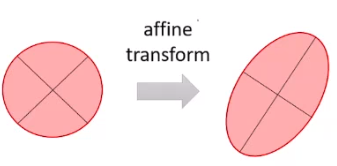
\includegraphics[scale=0.5]{8.png}
\end{center}
\paragraph{MSER} Maximally Stable Extremal Regions\\
Extract covariant regions (blobs) that are stable connected components of intensity sets of the image. Interesting areas stay the same at different threshold: stable with respect to variations in luminance, not scale dependent and doesn't assume circular regions. Key idea\ldots %TODO
Blobs generated (locally) by binarizing the image over a large number of thresholds %TODO
\subparagraph{Intuitions on MSER} Generate frames from the image by thresholding it on all graylevels.\\
Capture those regions that from a small seed of pixel grow to a stably connected region. Stability is assessed by looking at derivatives of region masks in time (most stable $\Rightarrow$ minima of connected region variation).
\paragraph{Image Segmentation} The process of partitioning an image into a set of homogeneous pixels, hoping to match objects or their subparts.\\
A naive approach: straighten the image in a $N\cdot M$ vector and use it as a dataset for K-means.\\
\subparagraph{Ncut} Normalized cuts
\begin{center}
	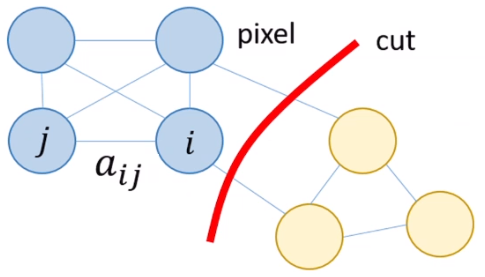
\includegraphics[scale=0.5]{9.png}
\end{center}
With each node being a pixel: an image is a graph. $a_{ij}$ is the affinity between pixels at a certain scale $\sigma$. A cut of $G$ is the set of edges such whose removal makes $G$ a disconnected graph. Breaking the graph into pieces by cutting edges of low affinity.\\
The normalized cut problem is NP-hard, approximate solution as an eigenvalue problem. But the eigenvalue decomposition it's really intractable with big images. We need to reduce the number of pixels. We can use \textbf{superpixels}: clustering the pixels with K-means (perhaps with different $K$) and using the clusters as nodes for segmentation algorithms (Ncut, Markov Random Fields\ldots). We can do multiscale superpixeling and segmenting at different scales, different policies\ldots\\
\subsubsection{Conclusion}
Image processing is a lot about convolutions: linear masks to perform gradient operations, gaussian functions to apply scale changes (zooming in and out). Computational efficiency is a driving factor: convolution in Fourier domain, superpixel, lightweight feature detectors\ldots
\subsection{Wavelets}
\paragraph{Limitations of DFT} Sometimes we might need localized frequencies rather than global frequency analysis.
\begin{center}
	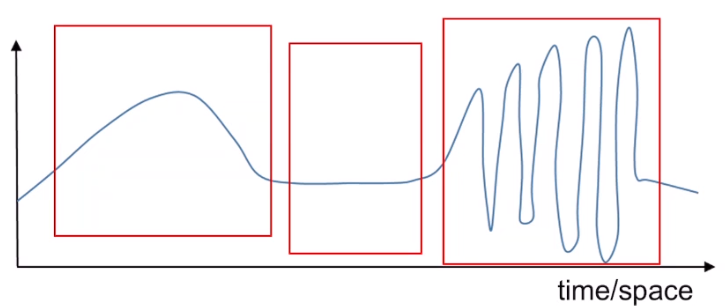
\includegraphics[scale=0.5]{10.png}
\end{center}
We slice the signal in "time slots" in time analysis and "frequency slots" in frequency analysis. In wavelet analysis you do both.\begin{center}
	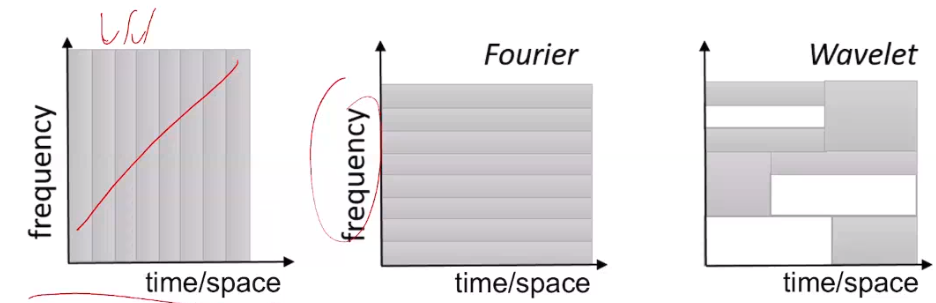
\includegraphics[scale=0.33]{11.png}\\
	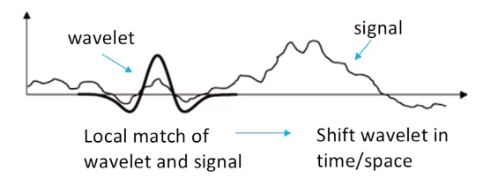
\includegraphics[scale=0.5]{12.png}
\end{center}
\begin{enumerate}
	\item Scale and shift original signal
	\item Compare signal to a wavelet
	\item Compute coefficient of similarity
\end{enumerate}
Split the signal with an orthonormal basis generate by translation and dilation of a mother wavelet $$\sum_t \hbox{x}(t)\phi_{j,k}(t)$$
Terms $k,j$ regulate scaling and shifting of the wavelet
$$\phi_{t,k}(\hbox{x}) = 2^{\frac{k}{2}}\phi\left(\frac{t-j2^k}{2^k}\right)$$
With many different options for the mother wavelet $\phi$
\begin{center}
	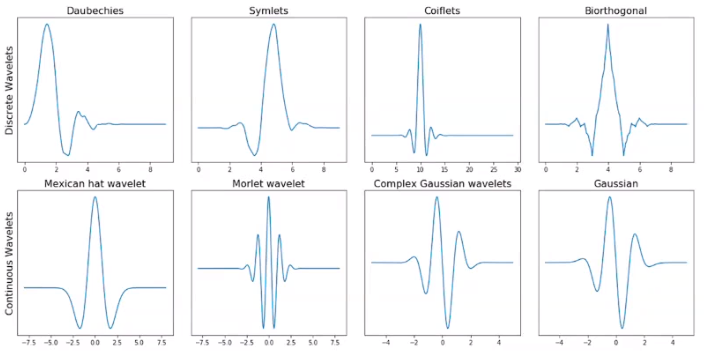
\includegraphics[scale=0.5]{13.png}
\end{center}
Scaling and dilation is akin to a sort of frequency: high scale mean stretched wavelet with slowly changing coarse feature and low frequency, while low scale compressed wavelet with rapidly changing details and high frequency.
\paragraph{DWT} Discrete Wavelet Transform: uses a finite set of scales and shifts rather than "any possible value" as in the continuous wavelet transform.
\section{Generative and Graphical Models}
Generative referring to the probability we learn: if we know the distribution probability of data we can generate new data.\\
Graphical referring to graphical formalisms that describe in a syntetic way the structures we'll see.
\paragraph{Generative Learning} ML models that represent knowledge inferred from data under the form of probabilities:
\begin{list}{}{}
	\item Probabilities can be sample: new data can be generated
	\item Supervised, unsupervised, weakly supervised tasks
	\item More easily incorporate prior knowledge on data and tasks
	\item Interpretable knowledge (how data is generated)
\end{list}
The majority of modern tasks comprises large number of variables\begin{list}{}{}
	\item Modeling the joint distribution of all variables can become impractical
	\item Exponential size of the parameter space
	\item Computationally impractical to train and predict
\end{list}
\paragraph{Representation} Graphical models are a compact way to represent exponentially large probability distributions. Encode conditional independence assumptions, and different classes of graph structures imply different assumptions/capabilities.
\paragraph{Inference} How to query (predict with) a graphical model? Probability of unknown $X$ given observations $d$, $P(X\:|\:d)$, the \textbf{most likely hypothesis} (parameters) $X$.
\paragraph{Learning} Find the right model parameters.
\paragraph{Representation} A graph whose nodes are random variables and edges represent probabilistic relationships between the variables.\\
Different classes of graphs:
\begin{list}{}{}
	\item Directed edges express \textbf{causal relationships}
	\item Undirected edges express \textbf{soft constraints}, values cannot change independently
	\item \textbf{Dynamic models}, graphs subject to structure changes to reflect dynamic processes. For example RNNs: recurrent neural networks are unfolded using weight sharing, producing a dynamic model.
\end{list}
\paragraph{In Deep Learning} Bayesian learning necessary to understand Variational Deep Learning.
\begin{center}
	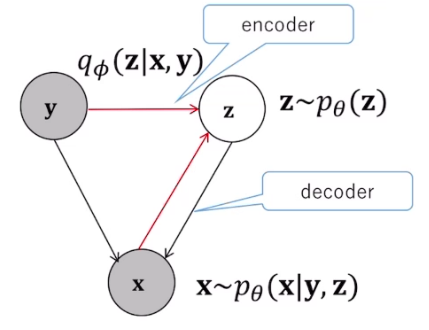
\includegraphics[scale=0.5]{14.png}
\end{center}
\paragraph{Generate new knowledge} Complex data can be generated if the model is powerful enough to capture its distribution.
\subsection{Probability Refresher}
\texttt{todo} %TODO
\subsubsection{Inference} Bayesian: consider all hypothesis weighted by their probabilities
$$P(X\:|\:d)=\sum_i P(X\:|\:h_i)P(h_i\:|\:d)$$
MAP (Maximum a-Posteriori): infer $X$ from $P(X\:|\:h_{MAP})$ where $h_{MAP}$ is the maximum a-posteriori hypothesys given $d$
$$h_{MAP} = \arg\max_{h\in H} P(h\:|\:d) = \arg\max_{h\in H} P(d\:|\:h)P(h)$$
ML assuming uniform prioris $P(h_i)=P(h_j)$ yields the maximum likelihood (ML) estimate $P(X\:|\:h_{ML})$ $$h_{ML} = \arg\max_{h\in H} P(d\:|\:h)$$
Any probability can be obtained from the Joint Probability Distribution $P(X_1,\ldots,X_n)$ by marginalization but at an exponential cost (e.g. $2^{n-1}$ for a marginal distribution from binary RV)
\subsection{Graphical Models}
Compact graphical representation for exponentially large joint distribution: simplifies marginalization and inference algorithms %TODO
\subsubsection{Bayesian Networks} 
\begin{multicols}{2}
Directed Acyclic Graphs (DAG) $G = (V,E)$\begin{list}{}{}
	\item Nodes $v\in V$ represent random variables\\
	Shaded $\Rightarrow$ observed, empty (like $Y_3$) $\Rightarrow$ unobserved
	\item Edges $e\in E$ describe the conditional independence relationships
\end{list}
\columnbreak
\begin{center}
	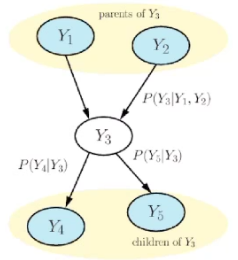
\includegraphics[scale=0.5]{15.png}
\end{center}
\end{multicols}
\paragraph{Conditional Probability Tables} CPTs are local to each node and describe the probability distribution \textbf{given its parents}.
$$P(Y_1,\ldots,Y_n) = \prod_{i=1}^N P(Y_i\:|\:\hbox{Parents}(Y_i))$$
\paragraph{Plate notation} If the same causal relationship is replicated for a number of variables, we can compactly represent it with plate notation.
$$P(Y_1,\ldots,Y_N,C) = P(C)\prod_{i=1}^N P(Y_i\:|\:C)$$
\begin{center}
	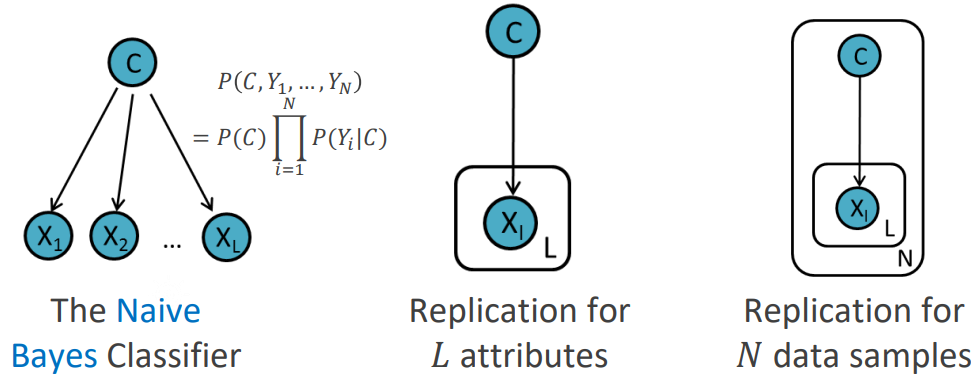
\includegraphics[scale=0.5]{16.png}
\end{center}
\paragraph{Full-Plate Notation}
Boxes denote replication for a number of times (denoted by the letter in the corner). Shaded nodes are observed variables, empty nodes are unobserved latent variables.\\
Black dots (optional) identify model parameters.
\begin{center}
	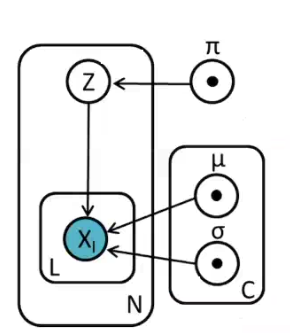
\includegraphics[scale=0.5]{17.png}
\end{center}
\subsubsection{Markov Random Fields}
\begin{center}
	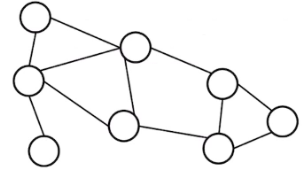
\includegraphics[scale=0.5]{18.png}
\end{center}
Undirected graph $G = (V,E)$ (a.k.a. Markov Networks). Also with shaded/empty nodes to denote observed/unobserved variables.\\
Edges $e\in E$ represent bidirectional dependencies between variables (constraints).\\
Often arranged in a structure that is coherent with the data/constraint we want to model.\\
Often used in image processing to impose spatial constraints (e.g. smoothness)
\subsection{Conditional Independence and Causality}
Can we reason on the structure of the graph to infer direct/indirect relationships between random variables?
\paragraph{Local Markov Property} Each node (random variable) is conditionally independent of all its non-descendants given a joint state of its parents. $$Y_v\perp Y_{V\setminus \hbox{Children(v)}}\hbox{ given }Y_{\hbox{Parent}(v)}\:\:\forall\:v\in V$$
There are substructures in the Bayesian networks with which we can build everything.
\paragraph{Markov Blanket} A Markov blanket $Mb(A)$ of a node $A$ is the minimal set of vertices that isolates/shields the node from the rest of the Bayesian network. If I know the variables in $Mb(A)$ then I know everything I need to know about $A$\begin{center}
	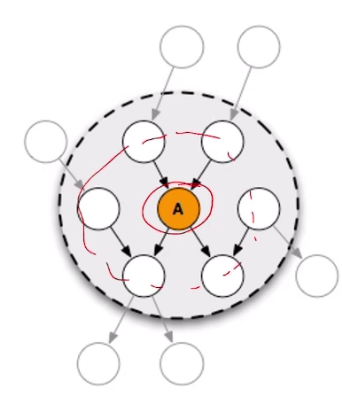
\includegraphics[scale=0.5]{19.png}
\end{center}
Taking only the parents it's not sufficient, we need also the children and the co-parents (nodes that are parents of one of my children). So it contains parents, children and children's parents.
$$P(A\:|\:Mb(A), Z) = P(A\:|\:Mb(A))\:\:\forall\:Z\not\in Mb(A)$$
\paragraph{Joint Probability Factorization} An application of the chain rule and local Markov property.\begin{enumerate}
	\item Pick a topological ordering of the nodes
	\item Apply chain rule following the order
\end{enumerate}
\paragraph{Sampling of a Bayesian Network} A BN describes a generative process for observations.
\begin{enumerate}
	\item Pick a topological ordering of the nodes
	\item Generate data by sampling from the local condition probabilities following this order
\end{enumerate}
Generate $i$th sample for each variable, example $s_i\simeq P(S)$, $h_i\simeq P(H\:|\:S=s_i)$
\subsection{Fundamental Bayesian Network Structures}
Three fundamental substructures that determine the conditional independence relationships in a Bayesian network. %TODO verify dependent/independent!!!!!
\paragraph{Tail to Tail} Common cause \begin{center}
	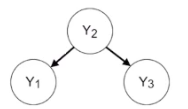
\includegraphics[scale=0.75]{20.png}
\end{center}
$$P(Y_1,Y_3\:|\:Y_2)=P(Y_1\:|\:Y_2)P(Y_3\:|\:Y_2)$$
If $Y_2$ is unobserved, then $Y_1,Y_3$ are marginally dependent $Y_1\not\perp Y_3$\\
If $Y_2$ is observed, $Y_1,Y_3$ become conditionally independent $Y_1\perp Y_3\:|\:Y_2$ (the path between $Y_1,Y_3$ is blocked by the observed (shaded) $Y_2$)
\paragraph{Head to Tail} \begin{center}
	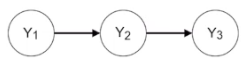
\includegraphics[scale=0.75]{21.png}
\end{center}
$$P(Y_1,Y_3\:|\:Y_2)=P(Y_1)P(Y_2\:|\:Y_1)P(Y_3\:|\:Y_2)=P(Y_1\:|\:Y_2)P(Y_3\:|\:Y_2)$$
Same behavior as before!\\
If $Y_2$ is unobserved, then $Y_1,Y_3$ are marginally dependent $Y_1\not\perp Y_3$\\
If $Y_2$ is observed, $Y_1,Y_3$ become conditionally independent $Y_1\perp Y_3\:|\:Y_2$ ($Y_2$ again blocks the path)
\paragraph{Heat to Head} Common effect\begin{center}
	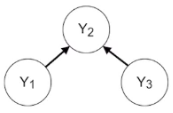
\includegraphics[scale=0.75]{22.png}
\end{center}
$$P(Y_1,Y_2,Y_3) = P(Y_1)P(Y_3)P(Y_2\:|\:Y_1,Y_3)$$
If $Y_2$ is unobserved, then $Y_1,Y_3$ are marginally independent $Y_1\perp Y_3$\\
If $Y_2$ is observed, then $Y_1,Y_3$ are conditionally dependent $Y_1\not\perp Y_3\:|\:Y_2$\\
If any $Y_2$ descendants is observed it unlocks the path.
\paragraph{Derived Conditional Independence Relationships} A Bayesian network represent the local relationship encoded by the 3 basic structures plus the derived relationships.
\end{document}